% !TeX root = Ausarbeitung_Anna-Lena_Marx.tex


%Laden des Datensatzes
%Exploration, Zusammenfassung und Visualisierung des Datensatzes
%Entwurf, Training und Test mehrer Modellarchitekturen
%Nutzung der Modelle, um Vorhersagen für neue Bilder zu treffen, und die Prognosegüte zu ermitteln.
%Zusammenfassung der Ergebnisse mit einem schriftlichen Bericht


\section{Maschinelles Lernen von belgischen Verkehrszeichen}
Diese Arbeit basiert auf dem belgischen Verkehrszeichen Datensatz (Belgian Traffic Sign Dataset) \cite{Timofte-MVA-2011}, der zum Training und zur Validierung des Modells genutzt werden soll. 
Der Datensatz für Training und Testing ist frei unter \url{https://btsd.ethz.ch/shareddata/BelgiumTSC/} verfügbar. \\
\\
Der Datensatz beeinhaltet Verkehrszeichen aus 62 Kategorien. Es handelt sich dabei also um eine Klassifikationsaufgabe, bei der jeweils ein einzelnes Bild eines Verkehrszeichen richtig zugeordnet werden soll. 
Im Rahmen dieser Hausarbeit sollen mit Hilfe des Frameworks \textit{Keras} mehrere Modelle von neuronalen Netzen entwickelt, mit dem Trainingsdatensatz trainiert und abschließend anhand ihrer Leistung aber auch der Architektur verglichen und bewertet werden. Abschließend soll die Leistungsfähigkeit der Modelle durch Bilder, die nicht dem Trainings- oder Testdatensatz angehören überprüft werden.

\section{Keras}
Keras wird als High-Level API für neuronale Netze beschrieben, die eine sehr einfache und schnelle Entwicklung dieser zum Ziel hat \cite{keras}. Das Framework selbst ist in Python geschrieben und nutzt TensorFlow \footnote{\url{https://www.tensorflow.org/}} (Google), CNTK \footnote{\url{https://github.com/Microsoft/cntk}} (Microsoft) oder Theano \footnote{\url{https://github.com/Theano/Theano}} (MILA, eingestellt) als Backend-Bibliothek für die eigentlichen Berechnungen. Keras selbst ist eine eigenständige Bibliothek und wird als solche entwickelt, gehört aber seit dem Release von TensorFlow 1.4 zur TensorFlow Core API. 
Wie auch TensorFlow ist Keras Open-Source und auf GitHub einsehbar.
Innerhalb dieser Arbeit wird Keras in der Version 2.2.2 mit TensorFlow 1.9.0 als Backend auf einer Linux-Plattform genutzt. \\
\\
Die Wahl von Keras als Framework ist durch die Klarheit und Verständlichkeit der API begründet. Dennoch steht mit TensorFlow eine bekannte, gut getestete und sehr mächtige Implementierung für maschinelles Lernen zur Verfügung. 
Für die Entwicklung und das Training wurde eine Intel(R) Core(TM) i7-7820HQ CPU mit 8 virtualisierten Kernen und 16 GB RAM verwendet. Auf eine für den Befehlssatz der CPU oder eine GPU optimierte Implementierung von TensorFlow wurde dabei verzichtet.

\section{Der Datensatz}
Der belgische Verkehrszeichen Datensatz unterscheidet zwischen 62 verschiedenen, aber teils sehr ähnlichen Kategorien. In den Abbildungen \ref{pic:vergleich-zeichen1} und \ref{pic:vergleich-zeichen2} ist dies anhand von Originalbildern aus den Trainingsdaten dargestellt. Während Bild (a) aus der Abbildung \ref{pic:vergleich-zeichen1} zwar Ähnlichkeiten mit den anderen beiden aufweist, ist es durch die Form klar abzugrenzen. Zwischen den Bildern (b) und (c) ist dies deutlich schwieriger. Bei Bild (b) handelt es sich um ein Gefahrenzeichen, während (c) ein rein informativen Charakter hat \cite{road-sign-defs}. Der Unterschied in Farbe und Form ist, gerade bei der Nutzung von Bildern in Graustufen nicht sehr groß. In der Anwendung einer künstlichen Intelligenz im Straßenverkehr ist die korrekte Unterscheidung zwischen Information und Gefahrenzeichen durchaus relevant. 
Noch deutlicher wird die Schwierigkeit in der Klassifikation in den unter Abbildung \ref{pic:vergleich-zeichen2} dargestellten Originalbildern. Es handelt sich tatsächlich um das selbe Zeichen, dass durch seine Ausrichtung eine gewisse Bedeutung erlangt. Der Datensatz unterscheidet zwischen \textit{mandatory direction (ahead)} (a) und \textit{mandatory direction (others)} (b und c). 
Damit ist die Klassifikation in diesem Fall von der Ausrichtung der Eingangsbilder abhängig. Schon bei einer leichten Verzerrung ist es denkbar, dass ein Modell zur Klassifikation die falsche Klasse auswählt. Dies wäre in der realen Welt aber auch bei einem menschlichen Fahrer leicht möglich, zeigt aber gut eine Schwierigkeit die aus dem Datensatz selbst resultiert.
%TODO ähnliche Kategorien Bilder

\begin{figure} [ht]
	\centering
	\subfloat[][]{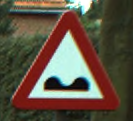
\includegraphics[width=0.2\linewidth]{0}}%
	\qquad
	\subfloat[][]{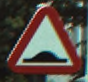
\includegraphics[width=0.2\linewidth]{1}}%
	\qquad
	\subfloat[][]{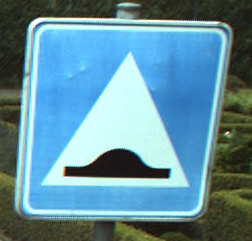
\includegraphics[width=0.2\linewidth]{59}}%
	\caption{(a) Klasse 0 \textit{Uneven road}, (b) Klasse 1 \textit{speed bump} , (c) Klasse 59 \textit{speed bump}}%
	\label{pic:vergleich-zeichen1}
\end{figure}

\begin{figure} [ht]
	\centering
	\subfloat[][]{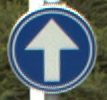
\includegraphics[width=0.2\linewidth]{34}}%
	\qquad
	\subfloat[][]{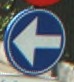
\includegraphics[width=0.2\linewidth]{35}}%
	\qquad
	\subfloat[][]{
\includegraphics[width=0.2\linewidth]{35-2}}%
	\caption{(a) Klasse 34 \textit{mandatory direction (ahead)}, (b) Klasse 35 \textit{mandatory direction (others)} , (c) Klasse 35 \textit{mandatory direction (others)}}%
	\label{pic:vergleich-zeichen2}
\end{figure} \ \\
%
Eine andere solche Schwierigkeit ist die Größe und Aufteilung des Datensatzes. Auf der schon genannten Website kann jeweils ein Trainings- und ein Testdatensatz heruntergeladen werden. Ein klar abgegrenzter Datensatz zur Validierung ist nicht verfügbar. Durch die Größe von Trainings- und Testdatensatz mit 4570 bzw. 2520 Bildern aufgeteilt sehr gering ist, kann nicht ohne weiteres ein Validierungsdatensatz abgetrennt werden. Auch die Aufteilung der Bilder im größeren Trainingsdatensatz erschwert dies. Abbildung \ref{pic:picsproclass} stellt die Problematik dabei gut dar. Während für 16 Klassen mindestens 100 Beispielbilder, anhand derer das neuronale Netz trainiert werden kann, vorhanden sind, müssen für 5 Klassen unter 10 Beispielbilder genügen. Machine Learning Verfahren leben von einer möglichst großen Datenmenge für das Training, es ist daher anzunehmen, dass für die 5 Klassen mit weniger als 10 Beispielbilder schlechtere Vorhersage-Ergebnisse als für die 16 Klassen mit mehr als 100 Beispielbildern erzielt werden. Zudem ist es auch hierdurch äußerst schwierig und wenig zielführend ein weiteren, distinkten Datensatz zur Verifikation abzugrenzen. 

\begin{figure} [ht]
	\centering
	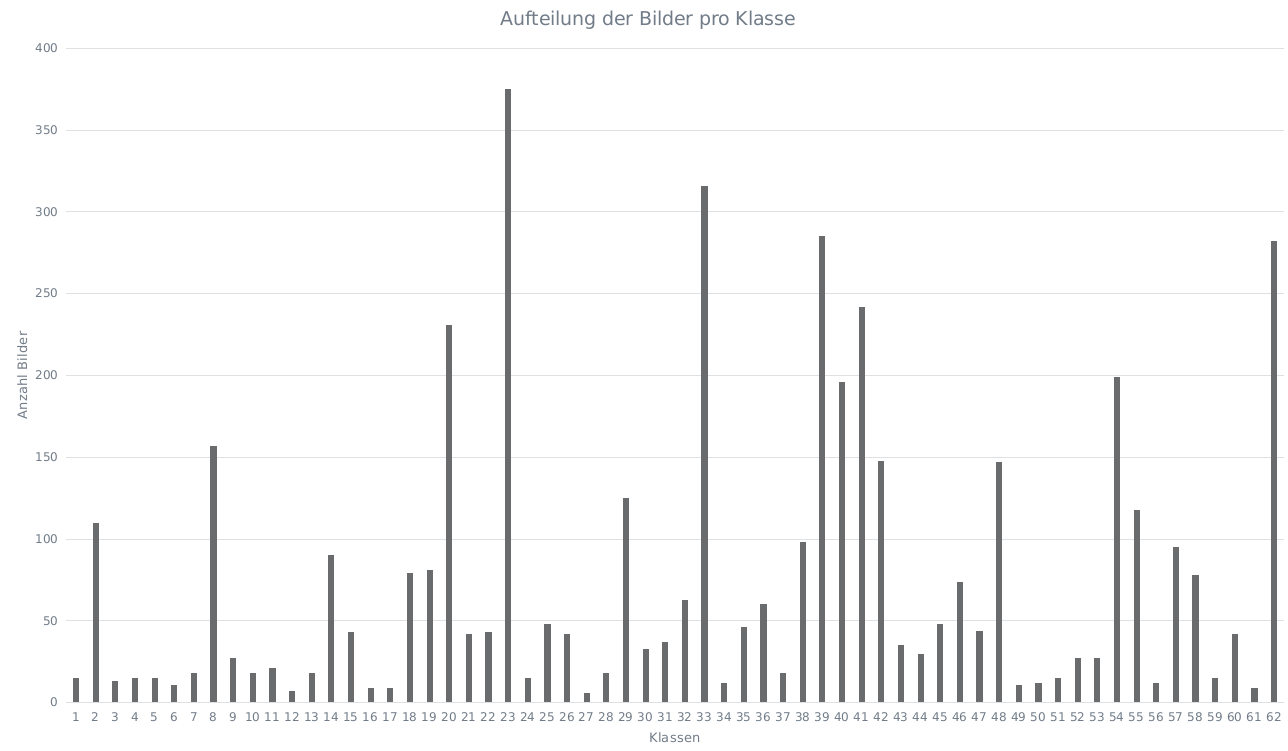
\includegraphics[width=\linewidth]{BilderProKlasse}
	\caption{Verteilung der Bilder pro Klasse für den Trainingsdatensatz}
	\label{pic:picsproclass}
\end{figure} \ \\
%
In den Abbildungen \ref{pic:vergleich-zeichen1} und \ref{pic:vergleich-zeichen2} werden bereits Beispielbilder aus dem Trainingsdatensatz dargestellt. Die Bilder liegen als Farbbilder (RGB) im PPM (Portable Pixmap) Format, aber in unterschiedlichen Bildgrößen vor. Die Bilder sind für Trainings- und Testdatensatz jeweils in Unterordnern, welche die Klassen repräsentieren, angeordnet. Zusätzlich befindet sich in jedem Unterordner eine CSV-Datei, die zusätzliche Informationen, wie die Breite, die Höhe, die Koordinaten der Region of Interest (ROI) und die Klassennummer, zu jedem Bildnamen enthält. Die Informationen aus dieser Datei wurden in dieser Arbeit nicht verwendet.

\section{Laden des Datensatzes}
Bevor die Datensätze für Training und Validierung zur weiteren Verwendung eingelesen werden können, müssen diese erst auf lokal gespeichert werden. Da dies in Python sehr einfach erledigt werden kann, soll an dieser Stelle nicht weiter darauf eingegangen werden. Im Quellcode \texttt{Keras.py} sind die entsprechenden Funktionen zum Herunterladen und entpacken der Datensätze in den Zeilen 23 bis 53 definiert. \\
\\
Ein Blick auf die Referenzimplementierung zu dieser Hausarbeit von Professor Volz zeigt den Aufwand, der in TensorFlow notwendig ist, um die Bilddaten zu laden und für das Verwendung in einem neuronalen Netz vorzubereiten. Keras kann diesen Prozess deutlich vereinfachen. Neben gewöhnlichem Laden der Daten bietet Keras mit der Klasse \texttt{ImageDataGenerator} und deren Methode \texttt{flow\_from\_directory} eine sehr einfache aber unheimlich mächtige Möglichkeit Bilddaten direkt aus einer Verzeichnisstruktur wie für den hier verwendeten Datensatz vorhanden auszulesen und für die weitere Verwendung vorzubereiten. Dies umfasst nicht nur gewöhnliches Preprocessing der Bilddaten, wie die Änderung und Vereinheitlichung der Bildgröße oder Ändern des Farbmodus, auch eine Echtzeit-Erweiterung des Datensatzes durch z.B. Verzerrung oder Rotation ist möglich. An dieser Stelle könnte auch eine Aufspaltung der Trainingsdaten in Trainings- und Testdatensätze erfolgen, aber aus den bereits im Abschnitt \textsc{Der Datensatz} genannten Gründen ist dies hier nicht sinnvoll.\\
\\
Die im folgenden Listing \ref{lst:load-data} abgebildete Methode stammt aus dem Quellcode \texttt{Keras.py} und zeigt, wie Trainings- und Validierungsdatensatz jeweils für das Training der neuronalen Netze geladen werden. \\
Ab Zeile 5 wird ein Objekt der Klasse \texttt{ImageDataGenerator} für die Generierung der Trainingsdaten angelegt. Bei diesen soll eine Erweiterung (Augmentation) der teils wenigen vorhandenen Bilder stattfinden, um eine breitere Datenbasis für das Training zu erreichen. Der erste Parameter, \texttt{rescale} gibt einen Skalierungsfaktor an, hat aber mit der Erweiterung der Datenbasis nichts zu tun. Diese wird über die folgenden Parameter \texttt{shear\_range}, \texttt{zoom\_range} und \texttt{horizontal\_flip} gesteuert. \\
Für die Validierungsdaten wird auf eine Erweiterung der Daten verzichtet, um die Resultate der Modelle vergleichbar mit anderen Ansätzen zu halten (Zeile 13).\\
\\
Das Laden der Bilddaten aus den Verzeichnissen erfolgt dann äquivalent für beide Datensätze über die Methode \texttt{flow\_from\_directory}, die auf dem jeweiligen \texttt{ImageDataGenerator} Objekt aufgerufen wird (ab Zeile 15 bzw. 22). Für beide wird zuerst der Pfad, von dem die Bilddateien geladen werden sollen angegeben, z.B. \texttt{/data/Training}. Mit dem nächsten Parameter, \texttt{target\_size} wird die Zielgröße der Bilder für, in diesem Fall, die Eingabe in ein neuronales Netz definiert. In dem beschriebenen Projekt wird eine Zielgröße von 32x32 Pixeln verwendet. Die \texttt{batch\_size} gibt an wie viele Bilddateien in einem Schritt verarbeitet werden sollen. Weiter könnte man über den Parameter \texttt{colormode} die Bilddaten zu Grauwertbildern konvertieren. Allerdings wurde die Entscheidung getroffen das Netz für diese Arbeit auf Basis von Farbbildern zu trainieren.

\begin{listing} [ht]
	\caption{Laden der Trainings- und Validierungsdatensätze}
	\label{lst:load-data}
	\begin{minted}[frame=lines, framesep=2mm, fontsize=\footnotesize, linenos]{python}
	def setup_data():
	#download_data()
	
	train_datagen = ImageDataGenerator(
	rescale=1. / 255,
	shear_range=0.3,
	zoom_range=0.3,
	horizontal_flip=True)
	
	valid_datagen = ImageDataGenerator(rescale=1. / 255)
	
	train_generator = train_datagen.flow_from_directory(
	train_data_dir,
	target_size=(img_width, img_height),
	batch_size=batch_size,
	#colormode='grayscale',
	class_mode='categorical')
	
	validation_generator = valid_datagen.flow_from_directory(
	validation_data_dir,
	target_size=(img_width, img_height),
	batch_size=batch_size,
	#color_mode='grayscale',
	class_mode='categorical')
	
	return train_generator, validation_generator
	\end{minted}
\end{listing} \ \\
%
Der letzte Parameter ist besonders wichtig, mit \texttt{class\_mode} wird angegeben, von welchem Typ das Label sein soll. Die korrekte Zuordnung dieses Modus zur Aufgabenstellung ist notwendig, um sinnvolle Ergebnisse aus der Arbeit mit einem Modell zu erhalten. Da es sich bei dem belgischen Verkehrszeichen Datensatz um ein Klassifizierungsproblem mit mehr als 2 Klassen handelt, sollte \textit{categorical} als Modus gewählt werden. \\
\\
Bei den Rückgabewerten (Zeile 29) handelt es sich um \texttt{DirectoryIterator} Objekte, die Tupel aus jeweils einem Batch aus Bilddateien und den zugehörigen Labeln enthalten. Diese können ohne weitere Transformationen für Training und Validierung der Modelle genutzt werden.\\
\\
Details zu den hier verwendeten Keras Methoden können in der API unter \url{https://keras.io/preprocessing/image/} und \url{https://keras.io/preprocessing/image/#imagedatagenerator-methods} nachgelesen werden.

\section{Entwurf der Modellarchitekturen}
%Layer an sich
%Architekturen für die einzelnen Netze

\section{Training der Modelle}

\section{Auswertung der Trainingsergebnisse}

\section{Vorhersagen für unbekannte Bilder}

\section{Zusammenfassung}

